\documentclass[UTF8]{ctexart}
\usepackage{listings}
\usepackage{textcomp} % 必须加上,否则报错
\usepackage{xcolor}
\usepackage{amsmath}
\pagestyle{plain}
\usepackage{fontspec}
\usepackage{graphicx}
\CTEXsetup[format={\Large\bfseries}]{section}
\lstset{language=Matlab}%代码语言使用的是matlab
\lstset{breaklines}%自动将长的代码行换行排版
\lstset{extendedchars=false}%解决代码跨页时,章节标题,页眉等汉字不显示的问题
\CTEXoptions[today=old] 
\title{Assignment 4}  %文章标题
\author{Zou Yuan\\Student No. 21960216}   %作者的名称
\date{Oct.18,2019}       %日期
\begin{document}
	\maketitle
	\section{P151, 3.1 Computer Problems: 3.}
	Write a Matlab function polyinterp.m that takes as input a set of (x,y) interpolating
	points and another $x_0$, and outputs $y_0$, the value of the interpolating polynomial at $x_0$. The first
	line of the file should be function $y_0 = polyinterp(x,y,x_0)$, where x and y are
	input vectors of data points. 

	The Matlab code is as follows:
	
	\begin{centering}
	\begin{lstlisting}
	
	function y0=polyinterp(x,y,x0)
	k=0;                       
	while(k<length(x)&&length(x)==length(y))                      
	k=k+1;                         
	c=newtdd(x,y,k);
	x1=-1:.01:4;
	y1=nest(k-1,c,x1,x);  
	y0=nest(k-1,c,x0,x);
	plot(x,y,'bo',x1,y1,x0,y0,'r--o')	
	end
	\end{lstlisting}
		\end{centering}
The input is:$$x =
1 \quad2\quad3\\$$$$y =
3.0000   \quad 5.6000 \quad   4.0000$$	
predictable point is $x_0=6$,The output is:
\begin{align*}
&ans =
-26.0000\\
\end{align*}

\section{P157, 3.2 Computer Problems: 1.}
   (a) Use the method of divided differences to find the degree 4 interpolating polynomial P4(x)
   for the data (0.6,1.433329), (0.7,1.632316), (0.8,1.896481), (0.9,2.247908), and
   (1.0,2.718282). (b) Calculate P4(0.82) and P4(0.98). (c) The preceding data come from the function $f (x) = e^{x^2}$. Use the interpolation error formula to find upper bounds for the error at
   x = 0.82 and x = 0.98, and compare the bounds with the actual error. (d) Plot the actual
   interpolation error $P(x) − e^{x^2} $on the intervals [.5,1] and [0,2].
   

   \begin{centering}
   	\begin{lstlisting}
   	
   	
   	x0=(0.6:0.1:1);
   	y0=[1.433329 1.632316 1.896481 2.247908 2.718282];
   	c=newtdd(x0,y0,5);
   	syms x y;
   	y=c(1)+c(2)*(x-x0(1))+c(3)*(x-x0(1))*(x-x0(2))...
   	+c(3)*(x-x0(1))*(x-x0(2))*(x-x0(3))+c(4)*(x-x0(1))*(x-x0(2))*(x-x0(4));
   	y=vpa(simplify(y),6);
   	disp(y)
   	x1=[0.82,0.98];
   	y1=zeros(1,length(x1));
   	r=zeros(1,length(x1));
   	tmp=ones(1,length(x1));
   	ff=diff(exp(x^5),5);
   	t=[-1:0.01:1];
   	a=zeros(1,length(t));
   	for i=1:2
   	y1(i)=nest(4,c,x1(i),x0);%拟合值
   	r(i)=abs(exp(x1(i)^2)-y1(i));
   	for j=1:4
   	tmp(i)=tmp(i)*(x1(i)-x0(j));
   	end
   	for k=1:length(t)
   	a(k)=subs(ff,t(k));
   	end
   	tmp(i)=abs(tmp(i)/factorial(5))*max(k);
   	end 
   	for i=1:2
   	fprintf('预测值%d:%d',i,y1(i))
   	fprintf('误差上界%d:%d',i,tmp(i))
   	end
   	t1=[0.5:0.01:1];
   	t2=[0:0.01:2];
   	ans1=nest(4,c,t1,x0);
   	ans2=nest(4,c,t2,x0);
   	hl1 = plot(t2,ans2,'-*r');
   	ax1 = gca;
   	set(ax1,'XColor','r','YColor','r')
   	ax2 = axes('Position',get(ax1,'Position'),...           
   	'XAxisLocation','top',...           
   	'YAxisLocation','right',...           
   	'Color','none',...           
   	'XColor','k','YColor','k');
   	hl2 = line(t1,ans1,'Color','b','Parent',ax2);
   	hl2.Marker='o';
   	
   	\end{lstlisting}   \end{centering}
   


The output is:
$$P_4(x) = 6.93957*x^3 - 11.6823*x^2 + 8.36355*x - 0.878137$$
\begin{centering}
预测值1:1.958910 \qquad 误差上界1:7.075200e-05\\
预测值2:2.612848 \qquad 误差上界2:2.566368e-03 \\
 \end{centering}
\begin{figure}[htbp]
 \begin{center}
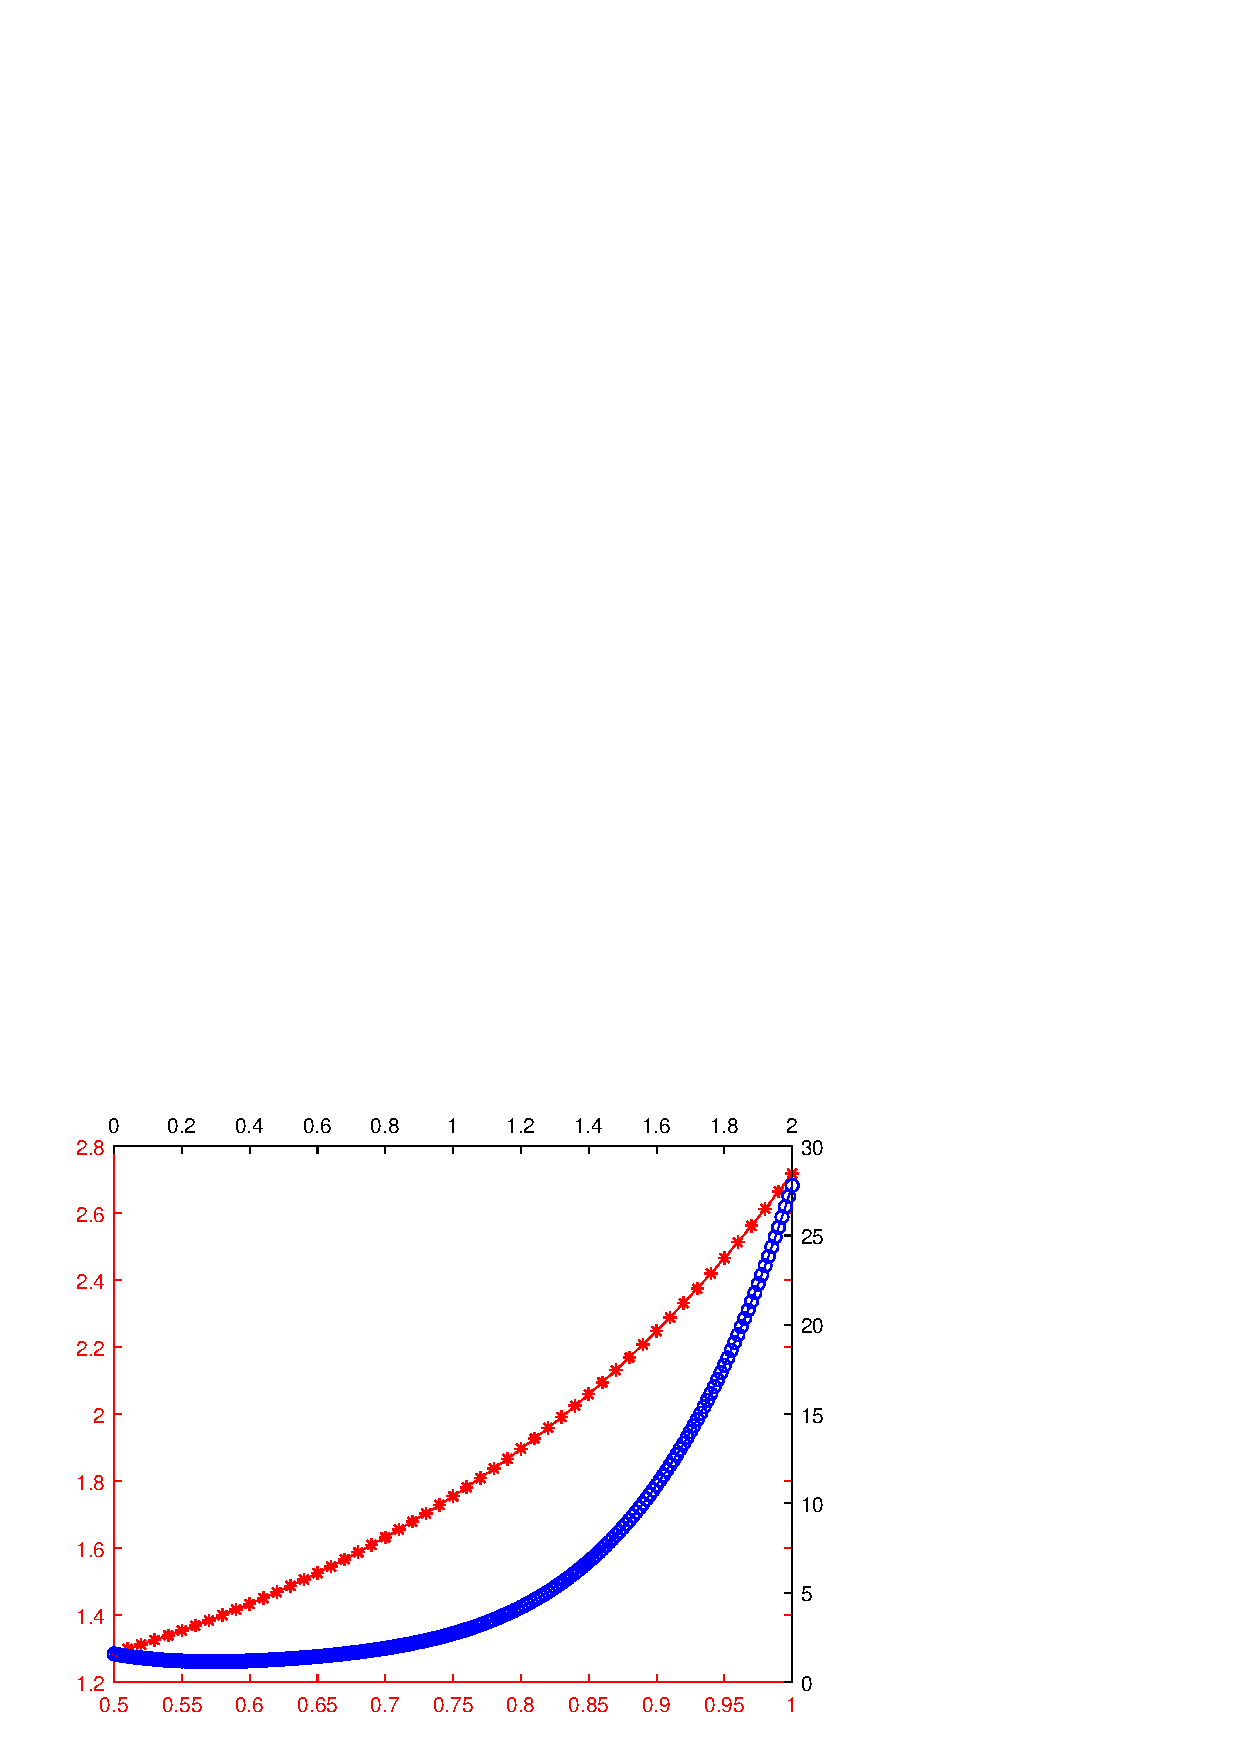
\includegraphics[scale=0.7]{./untitled.jpg}
\caption{Interpolation error on the intervals [.5,1] and [0,2]:}
\end{center}
\end{figure}
\section{P166, 3.3 Computer Problems: 2.}
Build a Matlab program to evaluate the cosine function correct to 10 decimal places using
Chebyshev interpolation. Start by interpolating on a fundamental domain [0,$\pi$/2], and extend
your answer to inputs between4 $10^{-4} $and $10^4$. You may want to use some of the Matlab code written in this chapter.

Code is below:
   \begin{centering}
	\begin{lstlisting}		
	function y=cos1(x)
	n=10;
	b=pi/4+(pi/4)*cos((1:2:2*n-1)*pi/(2*n));
	yb=cos(b);                     
	c=newtdd(b,yb,n);
	
	s=1;                           
	x1=mod(x,2*pi);
	if 3*pi/2>x1>pi/2
	x1 = abs(pi-x1);
	s = -1;
	end
	if x1 > 3*pi/2
	x1 = 2*pi-x1;
	end
	y = s*nest(n-1,c,x1,b);	
	\end{lstlisting}   
\end{centering}
\section{P178, 3.4 Computer Problems: 1.}
Find the equations and plot the natural cubic spline that interpolates the data points (a) (0,3),
(1,5), (2,4), (3,1) (b) (−1,3), (0,5), (3,1), (4,1), (5,1).
\begin{centering}
	\begin{lstlisting}	
	x0=[0 1 2 3];
	y0=[3 5 4 1];
	x1=[-1 0 3 4 5];
	y1=[3 5 1 1 1];
	splineplot(x0,y0,4)
	figure;
	splineplot(x1,y1,5)
	\end{lstlisting}   
\end{centering}
\begin{figure}[htbp]
	\begin{center}
		\includegraphics[scale=0.7]{./curve.jpg}
		\caption{Curve 1.}
	\end{center}
\end{figure}
\begin{figure}[htbp]
\begin{center}
	\includegraphics[scale=0.7]{./curve2.jpg}
	\caption{Curve 2.}
\end{center}
\end{figure}
\end{document}
